%%%% fatec-article.tex, 2024/03/10

%% Classe de documento
\documentclass[
  a4paper,%% Tamanho de papel: a4paper, letterpaper (^), etc.
  12pt,%% Tamanho de fonte: 10pt (^), 11pt, 12pt, etc.
  english,%% Idioma secundário (penúltimo) (>)
  brazilian,%% Idioma primário (último) (>)
]{article}

%% Pacotes utilizados
\usepackage[]{fatec-article}
\usepackage{float}

\Author{1}{Name={ Fagundes. L \\ Freitas. A \\ Freitas. V\\ Medina. L}}

\Author{2}{Name={\{ lucas.fagundes3@fatec.sp.gov.br \}\\ \{ amanda.freitas14@fatec.sp.gov.br \} \\ \{ valeria.freitas@fatec.sp.gov.br \} \\ \{ luiz.medina@fatec.sp.gov.br \}}}

%% Definição das palavras-chaves/keywords
\Keyword{1}{Citrus reticulata}{Citrus reticulata}
\Keyword{2}{Deficiência nutricional}{Nutritional deficiency}
\Keyword{3}{Visão computacional}{Computer Vision}
\Keyword{4}{Manganês}{Manganese}
\Keyword{5}{Cobre}{Copper}

%%%% Resumo no idioma primário (brazilian)
\begin{Abstract}[brazilian]%% Idioma (brazilian ou english)
  Este trabalho apresenta o desenvolvimento inicial do projeto NitrusLeaf, que utiliza técnicas de Inteligência Artificial (IA) para identificar deficiências nutricionais de cobre e manganês nas folhas da citrus reticulata (mexerica), alinhando-se com o Objetivo de Desenvolvimento Sustentável (ODS) 2 - Fome zero e agricultura sustentável da Agenda 2030 da ONU. O objetivo é reduzir as perdas na produção agrícola e promover a sustentabilidade. A aplicação visa facilitar aos agricultores a identificação desses problemas de forma rápida e precisa, utilizando visão computacional para analisar imagens das folhas, capturadas por drones ou enviadas pelos agricultores. A IA será treinada com o uso de redes neurais convolucionais (CNNs) utilizando um banco de dados de imagens de folhas com e sem deficiências. Espera-se que o NitrusLeaf se torne uma ferramenta eficaz para a agricultura sustentável após a conclusão desta pesquisa.  
\end{Abstract}

%%%% Resumo no idioma secundário (english)
\begin{Abstract}[english]%% Idioma (brazilian ou english)
  This work presents the initial development of the NitrusLeaf project, which utilizes specific Artificial Intelligence (AI) techniques to identify copper and manganese nutritional deficiencies in citrus reticulata (tangerine) leaves, with the aim of following the UN's 2030 Agenda, specifically Sustainable Development Goal (SDG) 2 Zero Hunger and Sustainable Agriculture, seeking to reduce agricultural production losses and promote sustainability. This application aims to help farmers identify these problems more easily and quickly, reducing tangerine crop losses and increasing plant health. Through computer vision, the system analyzes images of leaves, taken by drones or sent by farmers, and provides an accurate diagnosis. Convolutional Neural Networks (CNNs) will be used to train the AI with a database of images of leaves with and without deficiencies. After further research, it is expected that NitrusLeaf will become an effective tool for sustainable agriculture.
\end{Abstract}

%% Processamento de entradas (itens) do índice remissivo (makeindex)
\makeindex%

%% Arquivo(s) de referências
\addbibresource{fatec-article.bib}

%% Início do documento
\begin{document}

% Seções e subseções
%\section{Título de Seção Primária}%

%\subsection{Título de Seção Secundária}%

%\subsubsection{Título de Seção Terciária}%

%\paragraph{Título de seção quaternária}%

%\subparagraph{Título de seção quinária}%

\section*{Introdução}%
\label{sect:intro}
Vivemos em um mundo onde a comida não é suficiente para todos, e problemas como guerras e pobreza continuam a assolar diversas regiões. Esse mal perdura há muito tempo, e, em 1945, a Organização das Nações Unidas (ONU) foi criada para tentar combater esses desafios globais. Como parte dos esforços para enfrentar essas questões, a ONU lançou, em setembro de 2015, os Objetivos de Desenvolvimento Sustentável (ODS), definidos na Agenda 2030. Esse movimento global tem como metas principais erradicar a pobreza, proteger o meio ambiente e o clima, acabar com a fome e promover paz e prosperidade em todo o mundo. No presente projeto, buscamos reduzir as possíveis perdas de Citrus reticulata (mexerica), o que se alinha ao ODS 2 — Fome Zero e Agricultura Sustentável. Nosso foco é garantir uma maior produtividade das mexericas, contribuindo assim para a segurança alimentar e a sustentabilidade agrícola.\cite{IntroduçãoGreening}.

Atualmente, a taxa de produção de citros está diminuindo em todo o mundo, isso acontece por condições adversas de tempo ou por meio de pragas ou doenças que os citros podem vir a contrair, algumas das doenças são em nível global, como por exemplo a Phytophthora citrophthora, Xylella fastidiosa, cancro cítrico e o greening também conhecido como HLB e huanglongbing. No continente da América do Sul e América do Norte temos uma grande incidência do greening, isto pode ser visto por exemplo nos Estados Unidos que ano passado teve uma safra menor do que a normal por conta do greening e furacões \cite{IntroduçãoEUAProblemas}.

O Brasil também tem sua taxa de infecção por greening, esse greening é uma doença que ataca todos os tipos de citros e quando infectada a planta não tem cura, quando a planta infectada é nova elas não chegam a produzir frutos e as plantas adultas sofrem grande queda prematura dos frutos e definham ao longo do tempo. Uma das bactérias que causa essa doença no Brasil é a Candidatus Liberibacter asiaticus, Representando 99\% dos casos de greening , ela é a principal responsável pela doença. Essa bactéria é transmitida pelo psilídeo Diaphorina citri, também conhecido como Psilídeo-asiático-dos-citros, é um inseto de coloração branca acinzentada com manchas escuras nas asas, tem um comprimento de 2 a 3 mm e é muito frequente em pomares nas épocas de brotação das plantas. O estado de São Paulo também é habitado pelo greening, isso pode ser visto pelo Programa Nacional de Prevenção e Controle ao HLB (PNCHLB), que obriga a eliminação de plantas menores de oito anos que tenham contraído o HLB, ou seja, este problema também assola o vale do ribeira do estado de São Paulo \cite{IntroduçãoGreening}.

O HLB, popularmente conhecida como greening, tem como local de origem a Ásia há mais de 100 anos. Foi identificado no Brasil em 2004, nas regiões Centro e Leste do Estado de São Paulo, espalhando para todas as regiões citrícolas paulistas e pomares de Minas Gerais e Paraná, além de espalhar para a Argentina e Paraguai \cite{IntroduçãoGreening}.  

Por conta do greening ser uma doença que não tem cura, e após o descobrimento dela em um campo ser necessário a sua retirada para diminuir o risco de contaminações para as plantas ao redor, não há muito que possa ser feito para salvar a planta. Os sintomas do greening são folhas amareladas quando jovens e mosqueadas, apresentam pintas ou malhas escuras, quando maduras, além de que as folhas afetadas tendem a cair e em seu lugar nascer uma folha em posição vertical. Por conta disso a distinção entre o greening e outras doenças ou condições que tenham sintomas semelhantes é importante, para não se matar uma planta que pode ser salva. Duas das condições por deficiência de nutrientes que tem uma semelhança com os sintomas do greening são a deficiência de cobre e a de manganês. A deficiência de cobre tem como sintomas as folhas do fruto do novo ciclo de crescimento pequenas, deformadas e com nervuras verdes bem definidas sobre um fruto claro e as plantas podem apresentar folhas gigantes, bolsas de goma nos ramos novos e na casca dos frutos. Já a deficiência de manganês manifestam seus sintomas nas folhas novas, com um tamanho praticamente normal, perda de brilho e clorose, uma cor amarela esverdeada, entre as nervuras que permanecem verdes \cite{IntroduçãoGreening, IntroduçãoDeficiencias}.

São essas duas condições, as deficiências de cobre e manganês que nosso projeto busca analisar nas folhas da citrus reticulata. Foram escolhidas essas duas condições por terem um grau de semelhança com alguns dos sintomas do greening, como o amarelamento da folha e o crescimento diferente da folha. Nosso projeto busca verificar por meio de uma fota se a folha apresenta os sintomas de uma dessas duas deficiências de nutriente ou não. E com base nisso o agricultor pode aplicar as devidas medidas para combater os problemas, por meio da verificação do estado nutricional do solo em que a planta está plantada e com isso colocar os fertilizantes adequados no solo de maneira certa e balanceada.

Atualmente a Inteligência Artificial (IA) vem sendo utilizada em diversas área do mercado de trabalho, desde do ramo de saúde até os anúncios que vemos diariamente, sendo utilizada para aumentar a eficiência e qualidade, dando um resultado com maior exatidão em um número grande de situações. O objetivo das IA é pensar de forma autônoma e com respostas precisas para cada situação, sem ser necessário uma intervenção humana. Fazendo com que sua utilização em grandes empresas, hospitais e outros usuários que precisam automatizar algo, seja a cada dia maior e mais pronunciado.

O nosso sistema vai fazer uso  da IA para identificar a deficiência de manganês e cobre na folha da mexerica, a IA escanearia a foto e procuraria os sintomas das duas deficiências na folha, poderia ser uma folha com clorose, ou uma folha com coloração verde forte. Com base nisso ela identificaria e poderia retornar se a folha tem umas das duas deficiências, ou nenhuma delas.

A parte da IA que nosso projeto utilizara será a visão computacional, que tem como intuito permitir que a máquina veja visualmente e com base nisso identifique diversos dados pela imagem. Para poder ser utilizado a visão computacional primeiramente é necessário duas tecnologias chaves, rede neural convolucional e aprendizado de máquina profundo, popularmente conhecido como Deep Learning. São com essas duas ferramentas que se torna possível a máquina identificar certos padrões. A rede neural convolucional é usada em casos que há a necessidades de visão computacional, ela é inspirada na organização hierárquica do córtex visual humano,  construída com camadas intrinsecamente conectadas de estruturas de neurônios \cite{IntroduçãoRedeNeural}. No caso deep learning é uma tecnologia que chegou depois de machine learning, e é uma rede neural de multicamadas. Com deep learning é necessário apenas dizer se na imagem tem uma folha de citrus reticulata saudável ou uma com deficiência, e após enviar muitas imagens falando o que são cada uma ele iria descobrir o padrão. Já machine learning é necessário você por meio de programação descrever como é folha da planta saudável, falando sobre como seriam os pixels em uma imagem do padrão que você quer que a maquina reconheça \cite{IntroduçãoDeepLearning}.   

\section*{OBJETIVO} \label{sect:obj}

A agricultura de citros lida com diversos tipos de doenças nesta família, que são identificados a partir de observação de deformidades físicas e de pigmento em suas folhas, em sua casca e no fruto, além da presença de pragas no ambiente que afetam a qualidade final do alimento. A análise foliar é uma técnica comum usada para diagnosticar deficiências nutricionais em plantas, consistindo na coleta de folhas da planta, seguida pela análise química para determinar a concentração de determinados nutrientes. No entanto, por ser um processo que pode ser demorado e requer habilidades técnicas especializadas, e a utilização de IA na busca de padrões visuais facilitaria na determinação desse diagnóstico.

O projeto possui como objetivo o desenvolvimento de um sistema que seja capaz de reconhecer a deficiência dos nutrientes manganês e cobre da mexerica, a partir da análise de fotos de manchas em suas folhas com o auxílio da Inteligência Artificial, que através de padrões de identificação facilitará um possível diagnóstico diretamente para o agricultor produtor de mexerica. Os objetivos específicos são:
\begin{enumerate}
\item\textbf{Aprofundar na coleta de informações sobre os sintomas das deficiências de nutrientes específicos da mexerica.}
\item\textbf{Desenvolver um banco de imagens para estudo com uma variedade de níveis de deficiência de manganês e cobre para análise do problema;} 
\item\textbf{Realizar o treinamento da IA a partir do sistema de arquitetura de rede Neural Convolucional (CNNs).}
\item\textbf{Implementar um sistema que permita a identificação tecnicizada da deficiência usando Inteligência Artificial a partir de imagens digitais tiradas pelo próprio agricultor.}
\end{enumerate}

\section*{ESTADO DA ARTE} \label{sect:estadoarte}

Entre os muitos desafios enfrentados pelos agricultores, a deficiência de minerais nas plantas é uma preocupação significativa, pois pode resultar em perdas de produtividade e qualidade dos cultivos. A mexerica (Citrus reticulata) é uma das culturas suscetíveis a deficiências minerais, o que pode afetar seu crescimento, desenvolvimento e produção.

Recentemente, a inteligência artificial (IA) está sendo uma ferramenta poderosa para a detecção e diagnóstico de doenças e deficiência minerais em plantas. Com o uso de técnicas de aprendizado de máquina, visão computacional e análise de dados, surgiram aplicativos como o Plantix um aplicativo gratuito, desenvolvido por pesquisadores alemães, que faz a identificação de doenças em vários tipos de culturas com o uso da IA, o aplicativo foi referenciado no artigo \textcite{EstadoArte1}, como uma forma de identificar possíveis fitopatologias, que foi justamente a proposta do sistema que ele propôs. Um aplicativo mobile que auxilia na identificação de fitopatologias em diversas culturas, através de inteligência artificial.

Apesar de diversas semelhanças com o nosso projeto, há diferenças de objetivo, com o NitrusLeaf sendo focado na identificação de ausência de minerais na planta de mexerica através de uma analise por IA das folhas da planta, e a do artigo \textcite{EstadoArte1} sendo focado na identificação de fitopatologias em diversas culturas.

Pesquisadores têm utilizado câmeras de alta resolução e técnicas avançadas de processamento de imagens. Essas imagens são então analisadas por algoritmos de visão computacional para identificar padrões característicos associados a diferentes funções. O projeto de \textcite{EstadoArte2} busca fazer uma classificação de laranjas através de visão computacional para auxiliar na separação de laranjas ao comércio, invés do uso de peneiras que fazem a separação de laranjas grandes e pequenas. O sistema teve uma taxa de exatidão de 82\%, errando bastante na classificação de laranjas médias, porem mostra que a tecnologia tem uma grande eficácia. 

Já o nosso projeto é mais focado no cultivo e tratamento da planta, enquanto o projeto de \textcite{EstadoArte2} tem um foco no setor econômico e do comércio de laranjas, porem o nosso projeto também pode refletir nesses setores através de uma consequência dos nossos resultados, já que as árvores terão a produtividade esperada. Além do uso de visão computacional na identificação de deficiências minerais, que foi a mesma tecnologia utilizado no projeto de \textcite{EstadoArte2}, e seus resultados mostram que a eficácia dessa tecnologia é muito promissora.

O projeto de \textcite{EstadoArte3} utiliza também visão computacional com aprendizagem profunda, onde a proposta deles é detectar e classificar imagens de frutas, com o objetivo de fornecer informações nutricionais precisas com o uso de tabelas de composição alimentar. Utilizando um modelo inteligente baseado em CNN (Convolutional Neural Network) e Deep Learning. 

O projeto teve resultados excelentes com uma média de taxa de acerto de 96,5\% na identificação de bananas, maçãs e laranjas.

Com esses resultados mostra que um bom uso das tecnologias citadas, podemos chegar em um resultado satisfatório com o nosso projeto, onde grande parte dessas tecnologias vão ser a base do nosso projeto que busca, diferentemente dos outros projetos, dar uma função bastante complexa a máquina, que é a identificação da deficiência de minerais como o manganês e o cobre através da análise de imagens entregues pelos usuários.

\section*{METODOLOGIA} \label{sect:metodologia}

\section{Metodologia}

O desenvolvimento do projeto será conduzido em etapas que seguem a metodologia de desenvolvimento ágil (Scrum), permitindo uma adaptação flexível aos requisitos ao longo do processo. As etapas principais incluem:

\subsection{Coleta de requisitos e design}
Usaremos o Figma para desenvolver protótipos de baixa e alta fidelidade das interfaces da aplicação, garantindo uma visualização clara dos requisitos funcionais e de usabilidade.

\subsection{Desenvolvimento front-end}
O código será estruturado com HTML e CSS para a definição de layout e estilo, enquanto o JavaScript será utilizado para proporcionar interatividade. O \textit{Node.js} será empregado para a criação de componentes reutilizáveis, melhorando a eficiência e a modularidade do código.

\subsection{Desenvolvimento back-end e banco de dados}
O banco de dados será modelado no \textit{brModelo} e implementado no \textit{HeidiSQL} para garantir a correta estruturação dos dados. A interação entre \textit{front-end} e \textit{back-end} será implementada usando \textit{Python} para a integração da visão computacional e \textit{Node.js} no computador, enquanto o \textit{React Native} será utilizado para criar uma API no \textit{mobile}, com foco na criação de uma API eficiente.

\subsection{Testes e validação}
Após a implementação, serão realizados testes automatizados e manuais para validar o funcionamento correto de cada parte do sistema. Ferramentas como Selenium poderão ser utilizadas para automatizar os testes de interface.

\subsection{Publicação e acompanhamento}
O sistema será implementado na plataforma Web, sendo feito com \textit{front-end} e \textit{back-end} primeiramente, e em uma versão futura, algumas das funções disponíveis na Web serão adaptadas para \textit{mobile}, com o objetivo inicial de permitir o uso do aplicativo no campo para escanear a folha em tempo real e receber o feedback instantâneo. A fácil escalabilidade e manutenção serão garantidas, e ajustes serão feitos com base no feedback dos usuários após a implantação.

\section*{RESULTADOS PRELIMINARES}\label{sect:resultados}

Após aplicar os métodos descritos, foram alcançados os seguintes resultados: a prototipação das telas para dispositivos móveis utilizando o Figma, a criação do site com o Oracle APEX, a elaboração do Diagrama de Caso de Uso (DCU), o Escopo de Redes, a modelagem relacional e lógica do banco de dados (MBD), e o desenvolvimento do Modelo de Negócios Canvas.

\textbf{Prototipação do aplicativo no Figma}

A \Cref{fig:splash-screen} mostra a tela de splash screen do projeto, tendo a logo, a paleta de cores da identidade visual e a escolha do modo de entrada ou cadastro. Após logar ou se cadastrar você será levado à tela do inicio. 

\begin{figure}[H]
\centering
\caption{Splash Screen}%
\label{fig:splash-screen}
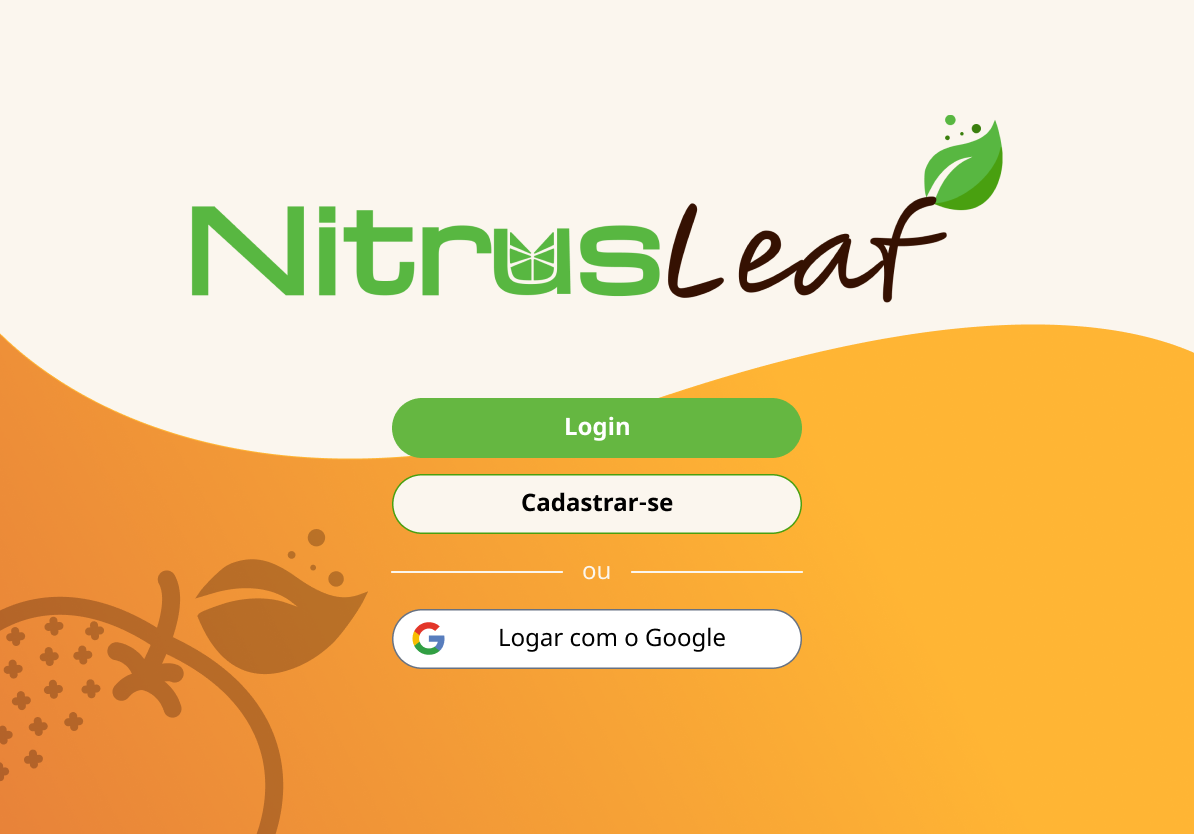
\includegraphics[width=0.8\linewidth]{Illustrations/Splash-Screen.png}
\SourceOrNote{Autoria Própria (2024)}
\end{figure}

A tela do inicio \Cref{fig:tela-inicio} oferece a opção de escanear a folha com o celular ou fazer o upload de uma imagem para escaneamento. Acima dessas duas opções encontra-se um quadrado contendo um gráfico de pizza que mostra a porcentagem da ocorrência das incidências, sendo amarelo manganês, laranja-avermelhado cobre e cinza adversos, que ocorre quando não há incidência de cobre nem de manganês. Um menu no canto esquerdo permite acessar outras telas do aplicativo, como histórico, drone e configurações gerais.

\begin{figure}[H]
\centering
\caption{Tela Início}%
\label{fig:tela-inicio}
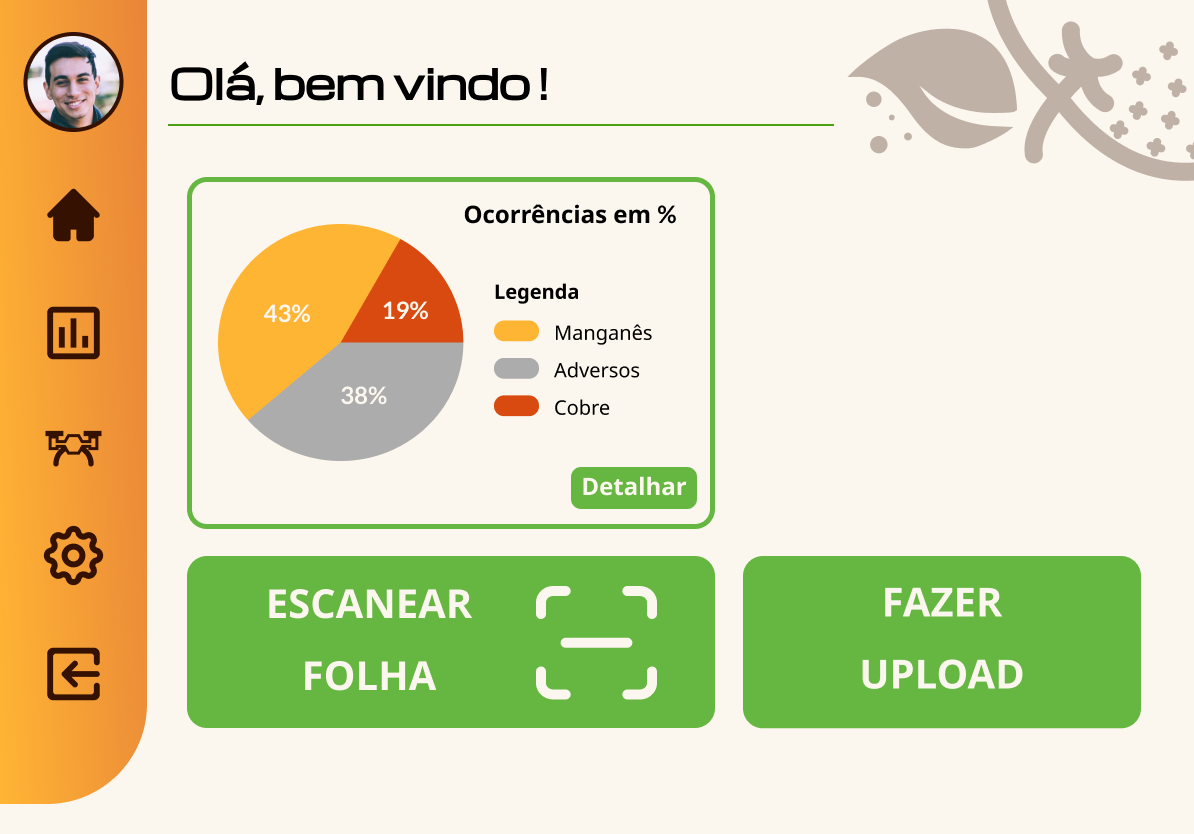
\includegraphics[width=0.8\linewidth]{Illustrations/tela-inicio.png}
\SourceOrNote{Autoria Própria (2024)}
\end{figure}

Ao apertar em escanear folha \Cref{fig:tela-escaneamento} será necessário apontar a câmera do celular para a folha escolhida e o aplicativo vai começar a escaneá-la e após terminar abrirá uma tela para você salvar a identificação da folha.


\begin{figure}[H]
\centering
\caption{Tela Escaneamento}%
\label{fig:tela-escaneamento}
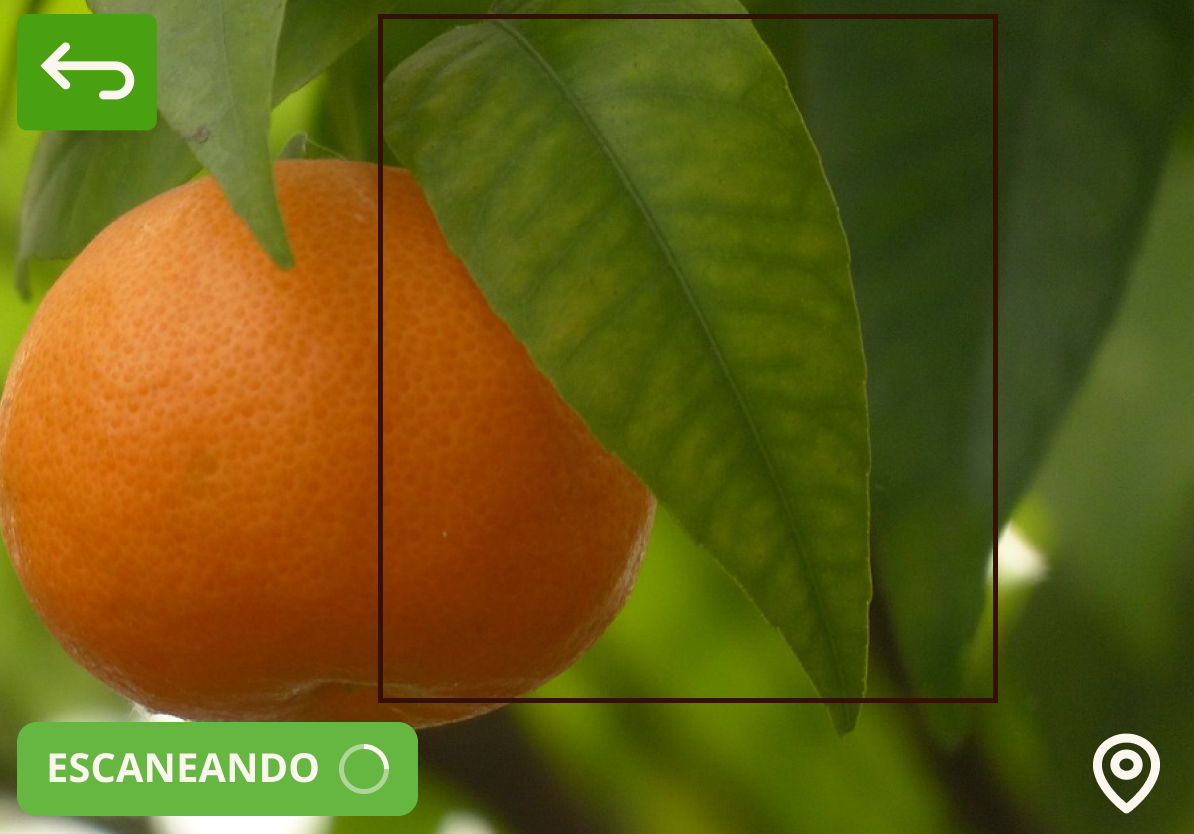
\includegraphics[width=0.8\linewidth]{Illustrations/Tela-Escaneamento.png}
\SourceOrNote{Autoria Própria (2024)}
\end{figure}

Após concluir o processo de escaneamento, o usuário será direcionado para uma tela onde poderá identificar o talhão correspondente à área escaneada, bem como o pé da folha que foi escaneada. Um talhão é uma área delimitada destinada ao plantio agrícola. Além disso, a tela mostrará a probabilidade de ser determinada uma deficiência, como ilustrado na \Cref{fig:cadastro-diagnóstico}. A opção de identificar da uma forma de controle para o usuário ter as informações de qual o pé que foi escaneado e o local em que ele foi escaneado salvas, possibilitando um maior controle para verificar se está tendo um grande número de incidências em um local específico.

\begin{figure}[H]
\centering
\caption{Cadastro Diagnóstico}%
\label{fig:cadastro-diagnóstico}
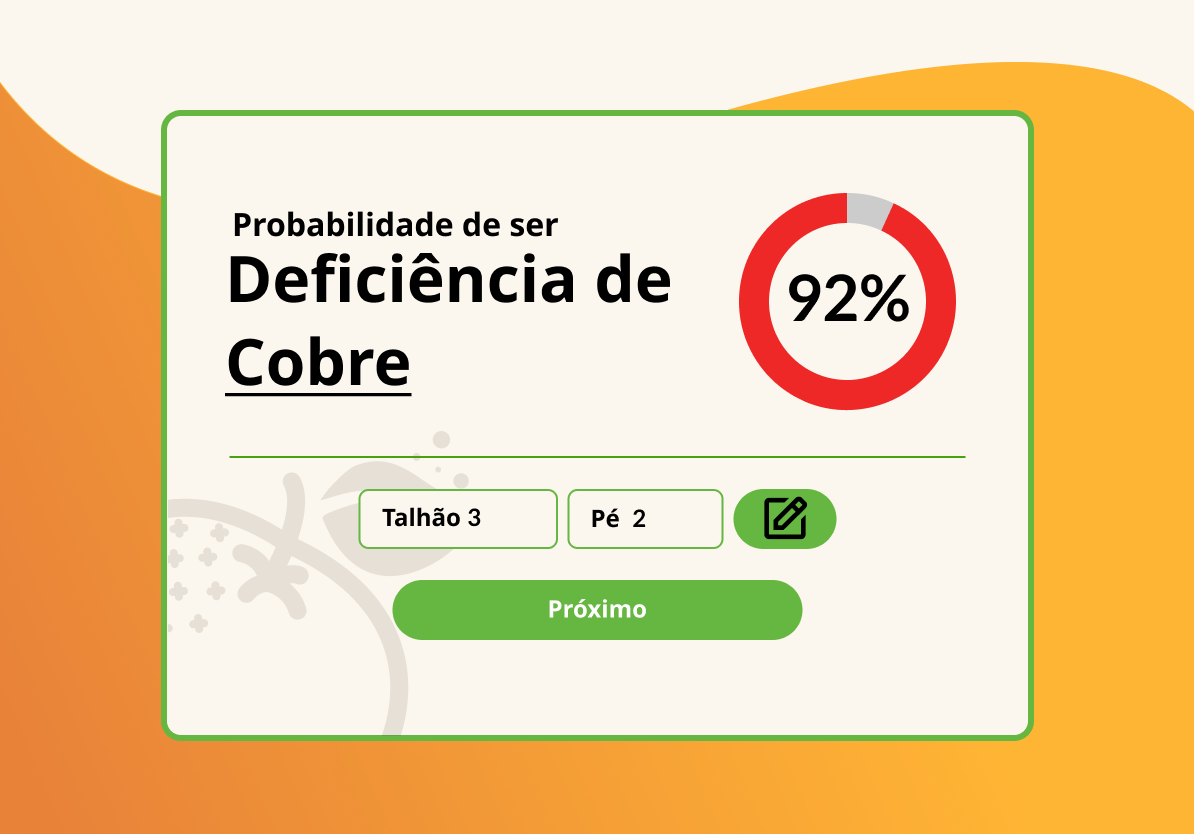
\includegraphics[width=0.8\linewidth]{Illustrations/Cadastro-diagnostico.png}
\SourceOrNote{Autoria Própria (2024)}
\end{figure}

Também a a tela com as informações tiradas dos drones \Cref{fig:tela-drone}, que seria o Índice de  estado de vegetação (NDVI) que é criado pelo drone ao tirar uma foto do local escolhido e um gráfico de linhas mostrando o nível do NDVI de cada talhão ao longo de 12 meses. O NDVI visa medir a quantidade de energia refletida e absorvida pelas plantas, fornecendo informações sobre sua saúde com base nessa reflectância. Na planta a parte de energia que é absorvida é o espectro da luz visível que vai de 400 a 720 nm (nanômetros), a parte que não é absorvida é a do espectro infravermelho próximo a luz visível, 720 a 1100 nm. As plantas saudáveis absorvem boa parte da luz visível e refletem fortemente o infravermelho próximo a luz visível. Já uma planta que está desidatrada, sofrendo de alguma doença ou algo que afete a sua saúde, absorvera mais da luz infravermelha. Logo o NDVI verificará a saúde das plantas por meio da refletividade das plantas. E de acordo com esse conhecimento terá uma fórmula que utilizará dos espectros que a planta reflete e absorve, (NIR) como a refletividade do infravermelho próximo e (VIS) como a refletividade vermelha. A fórmula é NIR menos o VIS dividido por NIR mais o VIS \cite{ResultadoNDVIArtigo, ResultadoNDVISite}.  

\[ NDVI =  \frac{NIR - VIS}{NIR + VIS} \]

A partir dessa fórmula, é obtido o valor do NDVI, que varia de -1 a 1. Variações com pequenos valores, como por exemplo os valores negativos, são geralmente associados a corpos d'água, enquanto valores acima de zero, que estão próximos dos valores negativos, representam nuvens. Os valores acima de 0,4 indicam a saúde das plantas, sendo os valores entre 0,6 e 0,8 considerados como representativos de plantas saudáveis. Essas informações são apresentadas na legenda na tela do mapeamento do drone.

\begin{figure}[H]
\centering
\caption{Tela Drone}%
\label{fig:tela-drone}
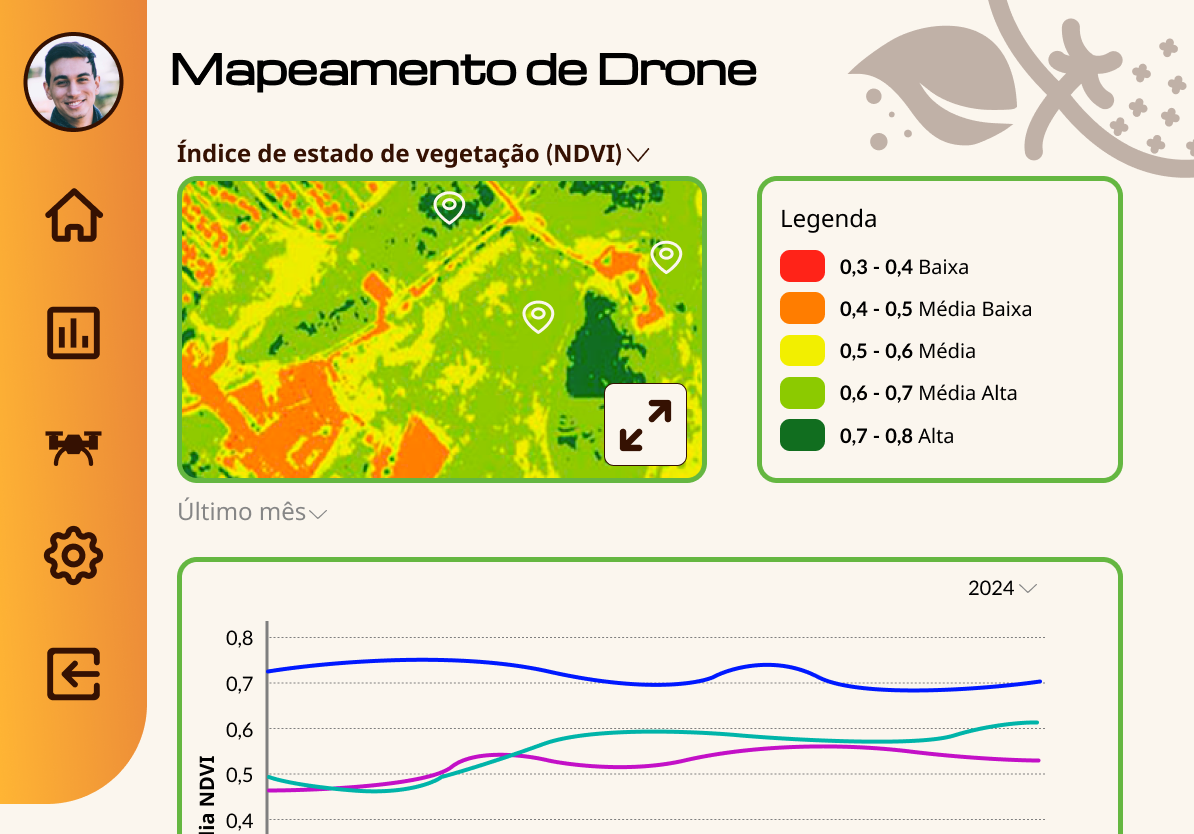
\includegraphics[width=0.8\linewidth]{Illustrations/tela-drone.png}
\SourceOrNote{Autoria Própria (2024)}
\end{figure}

Para verificar os pés cadastrados no aplicativo, acesse a tela de histórico \Cref{fig:tela-relatorios}. Nessa tela, você pode ver quantos pés estão cadastrados em cada talhão, bem como quantos pés do talhão foram analisados até o momento. No lado direito do histórico, uma janela de registros exibe o número total de talhões e pés registrados, assim como o número de pés analisados e diagnosticados.

\begin{figure}[H]
\centering
\caption{Tela Relatórios}%
\label{fig:tela-relatorios}
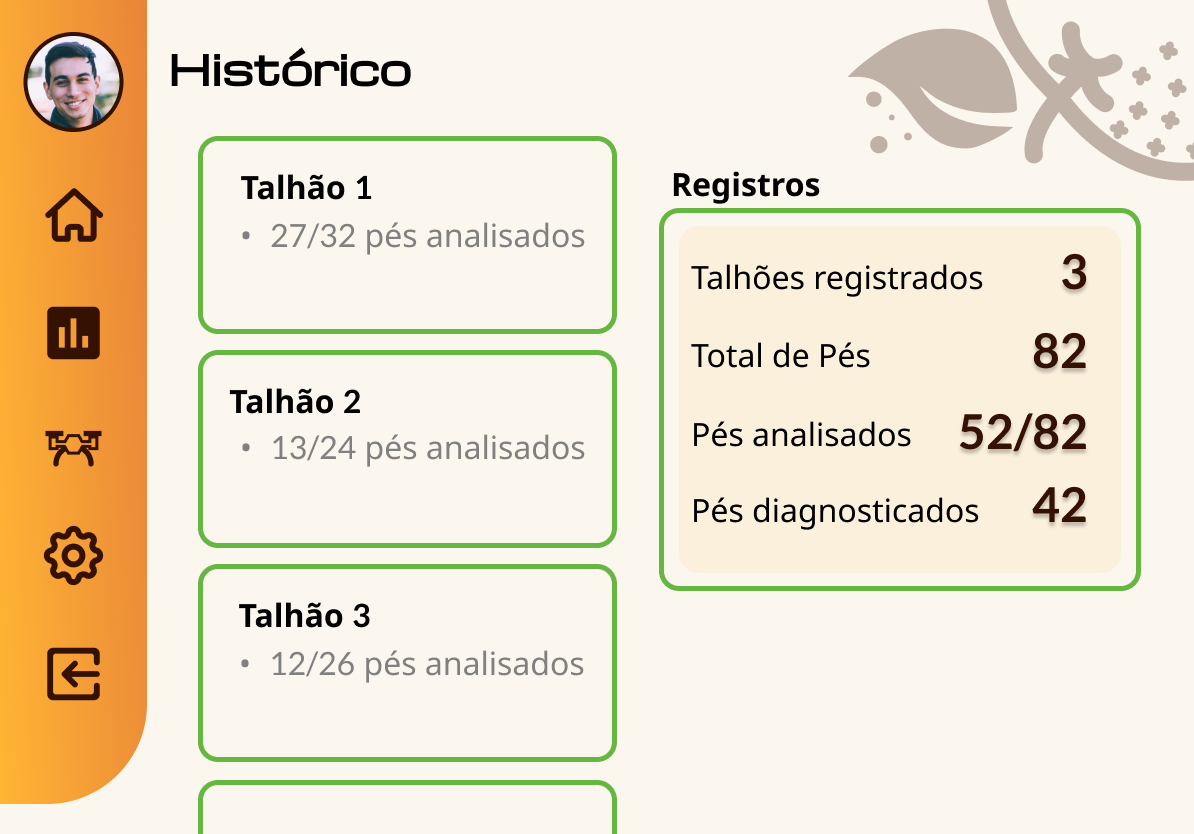
\includegraphics[width=0.8\linewidth]{Illustrations/tela-relatorios.png}
\SourceOrNote{Autoria Própria (2024)}
\end{figure}

\textbf{Oracle APEX}

Na aplicação desenvolvida no Oracle APEX, existem três telas principais. A primeira delas é a tela com o mapa, conforme ilustrado na \Cref{fig:APEX-mapa}. Esta tela exibe a localização exata de cada pé dentro dos talhões, fornecendo informações detalhadas sobre a incidência de condições, como deficiência de cobre, deficiência de manganês, ou nenhuma das duas, e identificando qual pé específico está sendo afetado.

\begin{figure}[H]
\centering
\caption{APEX Mapa}%
\label{fig:APEX-mapa}
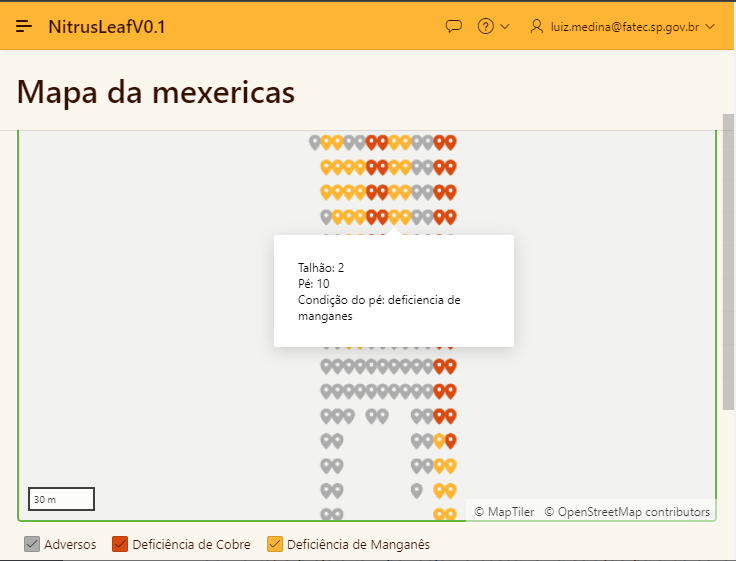
\includegraphics[width=0.8\linewidth]{Illustrations/mapa.png}
\SourceOrNote{Autoria Própria (2024)}
\end{figure}

A segunda tela da aplicação é a tela do mapa de calor, conforme ilustrado na \Cref{fig:APEX-mapa-de-calor}. Esta tela mostra a cor que identifica cada tipo de incidência e o nome correspondente. A concentração das cores aumenta conforme a proximidade das incidências. Por exemplo, se houver muitos casos de deficiência de manganês, eles estarão mais visíveis no mapa, permitindo a fácil identificação de grandes concentrações de deficiências nos locais.

\begin{figure}[H]
\centering
\caption{APEX Mapa de calor}%
\label{fig:APEX-mapa-de-calor}
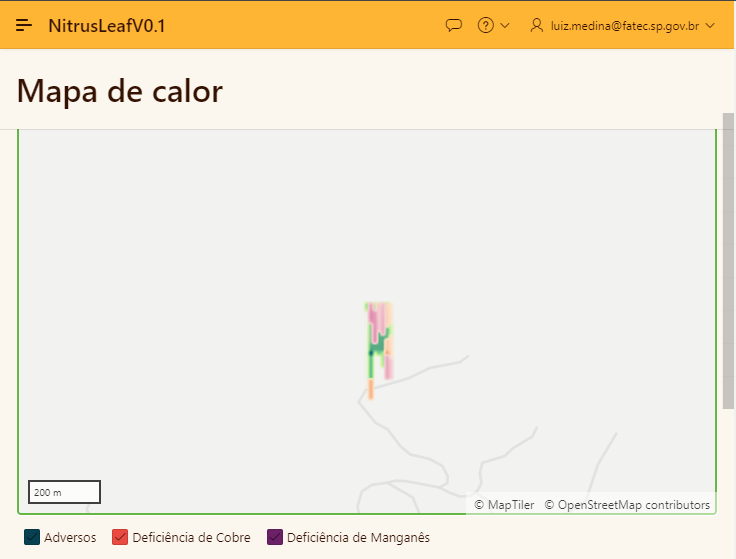
\includegraphics[width=0.8\linewidth]{Illustrations/mapadecalor.png}
\SourceOrNote{Autoria Própria (2024)}
\end{figure}

A última tela é a tela dos gráficos, conforme ilustrado na \Cref{fig:grafico}. Há dois gráficos: um gráfico de barras mostrando o número total de cada incidência e o número de pés que não apresentaram nenhuma das duas deficiências, categorizados como Adversos. O segundo gráfico é um gráfico de pizza, mostrando a porcentagem de cada incidência e a proporção de pés que não apresentam nenhuma das deficiências.

\begin{figure}[H]
\centering
\caption{APEX Gráficos}%
\label{fig:grafico}
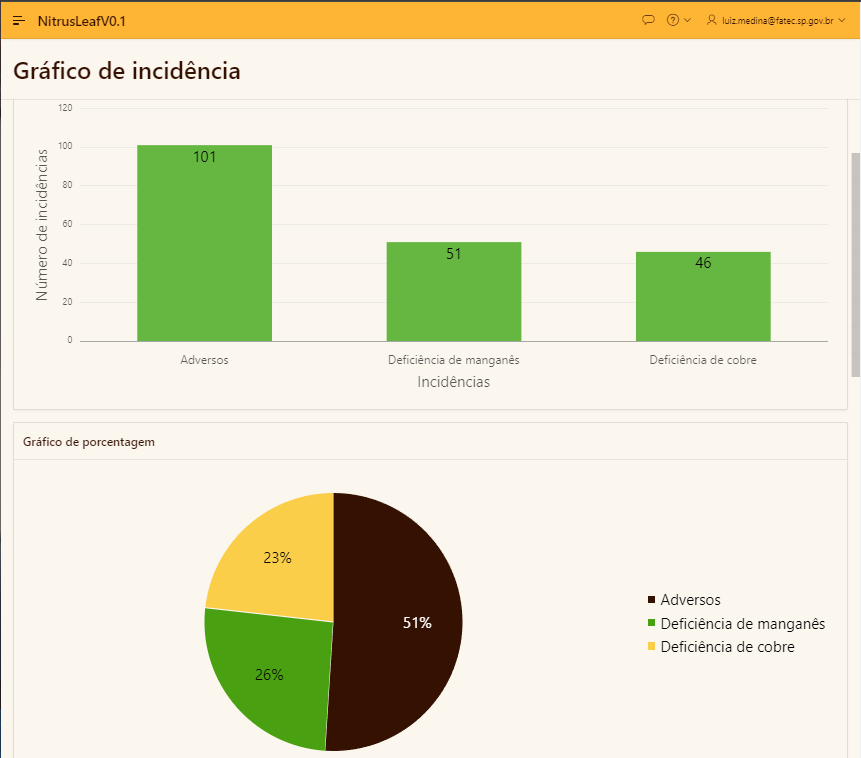
\includegraphics[width=0.8\linewidth]{Illustrations/grafico.png}
\SourceOrNote{Autoria Própria (2024)}
\end{figure}

\textbf{Diagrama de caso de uso (DCU)}

O DCU do projeto, ou Diagrama de Caso de Uso, é um diagrama utilizado para explicar as relações entre os atores (utilizadores do sistema) e as funcionalidades disponibilizadas pelo projeto. Conforme ilustrado na \Cref{fig:dcu}, ele mostra que o proprietário deve cadastrar as mexeriqueiras e, se desejar, cadastrar os drones. O funcionário é responsável por escanear as folhas, podendo fazer isso tanto com a câmera quanto fazendo upload das imagens. O aplicativo fornecerá o diagnóstico baseado nas imagens. Além disso, o funcionário pode consultar o mapa NDVI gerado pelo drone, bem como consultar o histórico e visualizar estatísticas. As funções do drone incluem tirar fotos do local e enviar um mapa NDVI.



\begin{figure}[H]
\centering
\caption{Diagrama de caso de uso (DCU)}%
\label{fig:dcu}
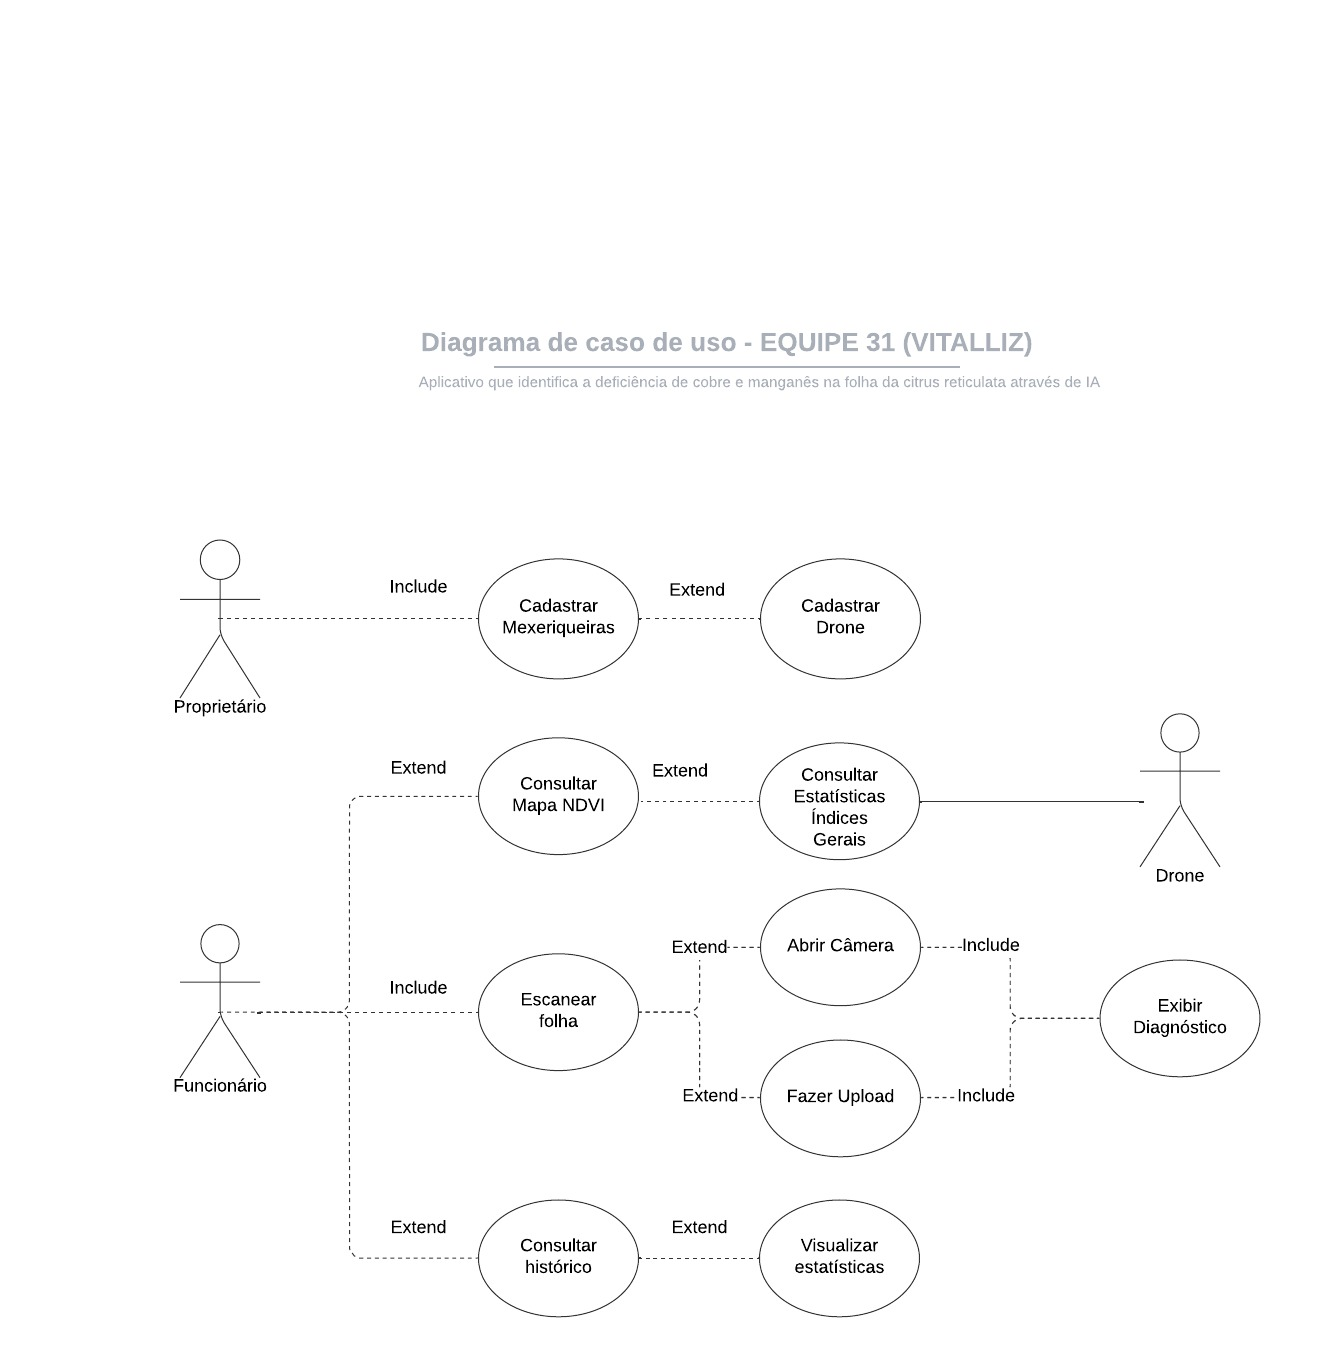
\includegraphics[width=0.8\linewidth]{Illustrations/dcu.jpeg}
\SourceOrNote{Autoria Própria (2024)}
\end{figure}

\textbf{Escopo de Redes}

A representação das ligações de rede do projeto é mostrada no escopo de redes, conforme ilustrado na \Cref{fig:escopoderedes}. Esta figura demonstra onde os programas são desenvolvidos e mantidos, sua conexão com a internet e o servidor, e a conexão do usuário com a internet. Quando o usuário envia fotos, estas passam pela internet e são armazenadas no servidor, que guarda as informações no banco de dados.

Os computadores estão todos conectados a um switch, que os conecta a um roteador. O roteador, por sua vez, os conecta à internet e, consequentemente, ao servidor. O roteador está localizado na área de manutenção.

Há também uma recepção, equipada com uma mesa para atender possíveis clientes. Nesta mesa, há um notebook conectado à internet via Wi-Fi, por meio de um modem com Wi-Fi que está situado na recepção.

\begin{figure}[H]
\centering
\caption{Escopo de Redes}%
\label{fig:escopoderedes}
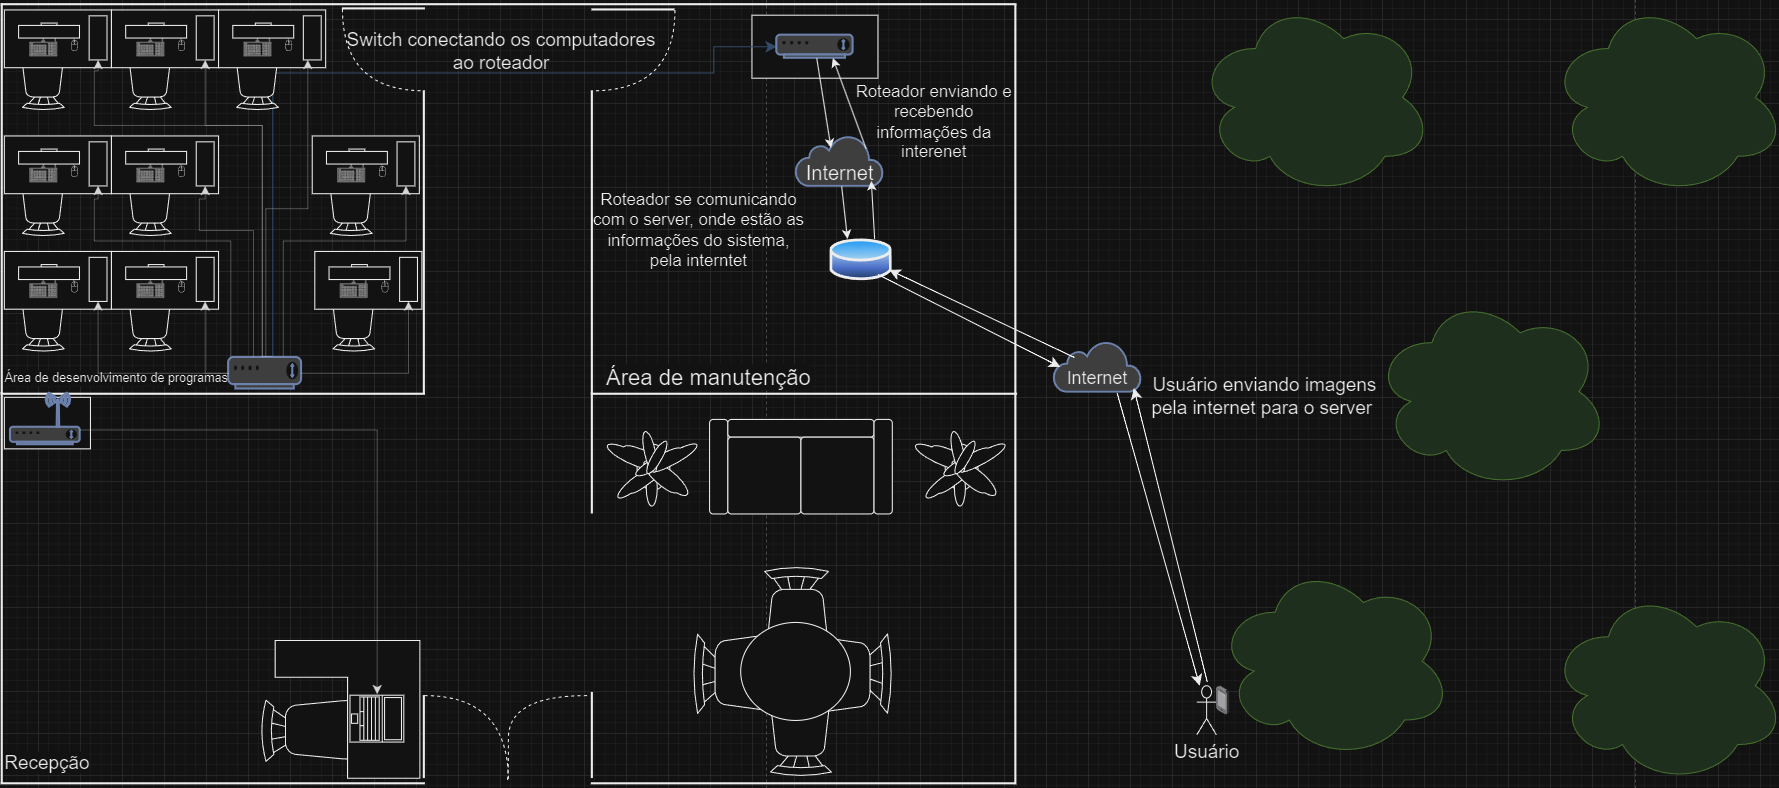
\includegraphics[width=0.8\linewidth]{Illustrations/escopoderedes.png}
\SourceOrNote{Autoria Própria (2024)}
\end{figure}

\textbf{Modelagem relacional e lógica do banco de dados}

A modelagem relacional do banco de dados \Cref{fig:mbdrelacional} do projeto NitrusLeaf tem como principal objetivo explicar a estrutura de dados utilizada para identificar deficiências nutricionais em folhas de mexeriqueira (Citrus reticulata). Este banco de dados é composto por várias entidades e seus respectivos relacionamentos, garantindo a integridade e a eficiência no armazenamento e consulta dos dados.

A entidade \textit{Folha} contém os atributos Id Fruta, Coloração Folhas, Tamanho e Nervuras, além de poder possuir três tipos de deficiência: manganês, cobre ou nenhuma deficiência. A entidade \textit{Foto} é considerada uma entidade fraca, utilizada para ligar a entidade \textit{Drone} e \textit{Folha}. \textit{Foto} possui os atributos Id\_Foto, Fk Id\_Drone (chave estrangeira que faz referência o drone), e Fk\_Id\_Fruta (chave estrangeira que referencia a folha).

A entidade \textit{Drone} tem os atributos Id\_Drone, Visibilidade, Qualidade e Capacidade. \textit{Drone} é responsável por gerar a entidade \textit{Imagem}, que possui os atributos Id\_Imagem, fk\_id\_Drone, Nitidez e Visibilidade. \textit{Imagem} é utilizada para identificar a coloração da folha através da entidade \textit{Coloração} e também gera a entidade \textit{Diagnóstico}. \textit{Diagnóstico} possui os atributos Id\_Diagnóstico, Fk\_Id\_Imagem (chave estrangeira que faz referência a imagem) e Qtd\_Historico. Em seguida, \textit{Diagnóstico} gera a entidade \textit{Histórico}, que contém os atributos Id\_Histórico, Data\_Emissão e Capacidade\_Armazem.

A entidade \textit{Imagem x Produtor} serve para relacionar a imagem com o produtor, possuindo os atributos Id\_ImgXProd, Fk\_Id\_Imagem e Fk\_Id\_Produtor. A entidade \textit{Produtor} tem os atributos Id\_Produtor e Nome, e interage com as entidades \textit{Email}, \textit{Telefone} e \textit{Login}. \textit{Email} possui os atributos Id\_Email, Fk\_Id\_Produtor e Correio\_eletrônico. \textit{Telefone} contém os atributos Id\_Telefone, Fk\_Id\_Produtor e Número, permitindo que o produtor tenha múltiplos números de contato. Por fim, a entidade \textit{Login} possui os atributos Id\_Login, Usuário e Senha.

\begin{figure}[H]
    \centering
    \caption{Modelo Relacional do Banco de Dados}%
    \label{fig:mbdrelacional}
    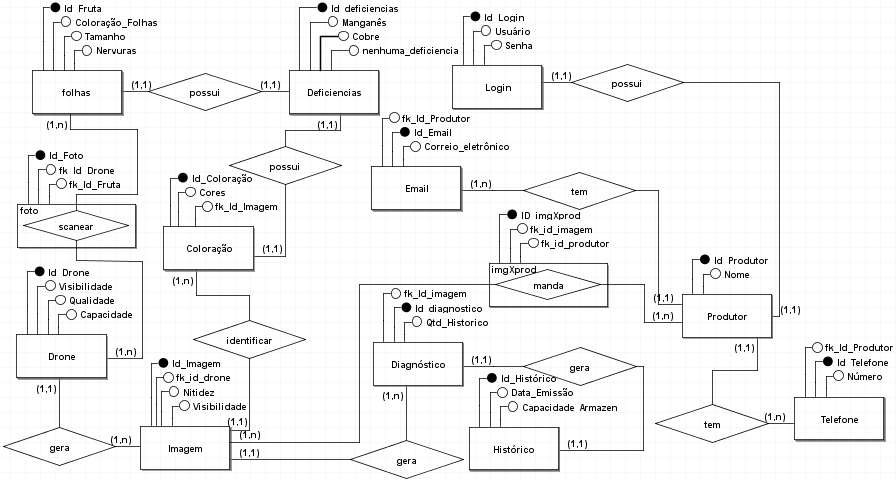
\includegraphics[width=0.8\linewidth]{Illustrations/mbdrelacional.png}
    \SourceOrNote{Autoria Própria (2024)}
    \end{figure}

Esse modelo relacional detalha como o banco de dados é estruturado para garantir a gestão eficiente das informações no aplicativo NitrusLeaf. Ele permite a identificação precisa de deficiências nutricionais nas folhas de mexeriqueira, suportando as funcionalidades do aplicativo, desde a captura de fotos pelos drones até a geração de diagnósticos e armazenamento de históricos. A estrutura relacional assegura que as informações sejam bem organizadas e facilmente acessíveis, otimizando o processo de recuperação das plantas e ajudando os produtores a evitar a perda de frutos. Além do modelo relacional, também há o modelo lógico mostrado na \Cref{fig:mbdlogico}.

\begin{figure}[H]
\centering
\caption{Modelo Lógico do Banco de Dados}%
\label{fig:mbdlogico}
\includegraphics[width=0.8\linewidth]{Illustrations/mbdlógico.png}
\SourceOrNote{Autoria Própria (2024)}
\end{figure}

\textbf{Modelo de negócios Canvas}

O modelo de negócios Canvas do projeto NitrusLeaf \Cref{fig:canvaspi} tem como principal objetivo delinear os elementos cruciais para o sucesso do nosso empreendimento. Esse modelo abrange várias áreas essenciais, incluindo nossos parceiros, proposta de valor, relacionamento com o cliente, recursos e atividades chave, canais, estrutura de custos e fontes de renda.

Parceiros Chave

Nosso foco principal em parceiros chave são os locais e entidades envolvidas no setor agrícola, especialmente aqueles interessados em inovação tecnológica. Esses parceiros incluem cooperativas agrícolas, universidades, centros de pesquisa, empresas de tecnologia agrícola, secretarias de agricultura dos municípios do Vale do Ribeira e associações de fazendeiros. A colaboração com esses parceiros é fundamental para ampliar o alcance do projeto e assegurar suporte técnico e científico.

Proposta de Valor

A proposta de valor do NitrusLeaf gira em torno da capacidade de identificar deficiências nutricionais nas plantas, especificamente a falta de manganês e cobre nas folhas de mexerica, de maneira eficiente e em tempo real. Além disso, o projeto visa manter um padrão elevado de qualidade dos frutos, ajudando os agricultores a otimizar a saúde das plantas e a produtividade.

Relacionamento com o Cliente

O relacionamento com o cliente é focado em oferecer um suporte abrangente. Isso inclui suporte técnico para a utilização do aplicativo via WhatsApp e feedback do cliente pelo app, além de canais de comunicação para feedback e resolução de dúvidas. Nosso objetivo é garantir que os clientes se sintam apoiados e possam maximizar os benefícios do nosso sistema.

Recursos Chave

Os recursos chave para o desenvolvimento e operação do NitrusLeaf incluem infraestrutura tecnológica (servidores, drones, câmeras de alta resolução), conhecimento técnico em agronomia e TI, uma equipe de suporte dedicada, programadores, instaladores do sistema físico, funcionários para suporte online e host para hospedar o site. Esses recursos são essenciais para o funcionamento eficaz do sistema.

Atividades Chave

As atividades chave do projeto incluem o desenvolvimento contínuo do software, a calibração dos algoritmos de IA para identificar deficiências nutricionais, a manutenção dos drones e outros equipamentos, e a realização de testes de campo para validar os diagnósticos fornecidos pelo sistema.

Canais

Os canais através dos quais promovemos e oferecemos nossos serviços incluem nosso website, redes sociais, feiras agrícolas, eventos de tecnologia, newsletters, parcerias com distribuidores agrícolas e anúncios pelas secretarias de agricultura dos municípios do Vale do Ribeira.

Estrutura de Custos

A estrutura de custos engloba despesas com desenvolvimento e manutenção do software, compra e manutenção de equipamentos (drones e câmeras), marketing e promoção, salários da equipe, custos operacionais gerais como servidores e infraestrutura de TI, manutenção dos itens que realizam o monitoramento das mexericas, compra dos produtos necessários para o monitoramento, host para hospedar as informações, aluguel do sistema e itens necessários, e mão de obra para instalação e manutenção.

Fontes de Renda

A principal fonte de renda do NitrusLeaf provém da venda de assinaturas para o uso do aplicativo, serviços de análise de solo e plantas, consultoria técnica, parcerias com empresas e aluguel do sistema.

Em resumo, o modelo de negócios Canvas do NitrusLeaf oferece uma visão abrangente de como estruturamos nosso projeto para atingir nossos objetivos e atender às necessidades dos nossos clientes. Nossa abordagem integrada garante que todos os aspectos do negócio estejam alinhados para promover a saúde e produtividade das plantações de nossos usuários.

\section*{CONCLUSÃO}\label{sect:conclusao}

Inicialmente, o projeto tem por objetivo buscar uma solução para as deficiências de minerais encontradas na mexeriqueira (Citrus reticulata), especificamente na variedade conhecida como mexerica, e, consequentemente, apresentar uma alternativa ao problema utilizando tecnologia. Dessa forma, elaboramos um projeto cuja ideia central é criar uma aplicação capaz de identificar, em tempo real, a deficiência de minerais pela qual a planta está passando. Isso permitirá produzir um diagnóstico preciso, facilitando o processo de recuperação da planta, evitando a perda de frutos e otimizando o tempo dos produtores.

Diante disso, nos deparamos com algumas limitações ao longo da pesquisa, pois ela é restrita a apenas alguns países e às condições do solo. A falta de minerais na planta possui relação direta com a acidez do solo. Nosso estudo tem por objetivo identificar especificamente deficiências de manganês e cobre em plantas de Citrus reticulata (mexerica) através da análise foliar. Pesquisas mostram que uma planta com deficiência de manganês geralmente não apresenta deficiência de cobre e vice-versa. Uma análise mais aprofundada revela que a deficiência está diretamente ligada ao pH do solo. A carência de manganês pode ser identificada em um solo mais ácido, enquanto a deficiência de cobre pode se manifestar em um solo alcalino \cite{ConclusãoMicroN, ConclusãoCobre}.

\printbibliography

%% Elementos pós-textuais (opcionais): Apêndice e Anexo
%Caso for utilizar, basta retirar o símbolo de % na frente do comando
%%%%% Elementos pós-textuais
%%
%% Glossário, apêndices, anexos e índice remissivo (opcionais).

%% Apêndices
\begin{Appendix}

    \section{Modelo de negócios Canvas}%
    \label{sect:apx-a1}
    
    \begin{figure}[H]
    \centering
    \caption{Modelo de negócios Canvas}%
    \label{fig:canvaspi}
    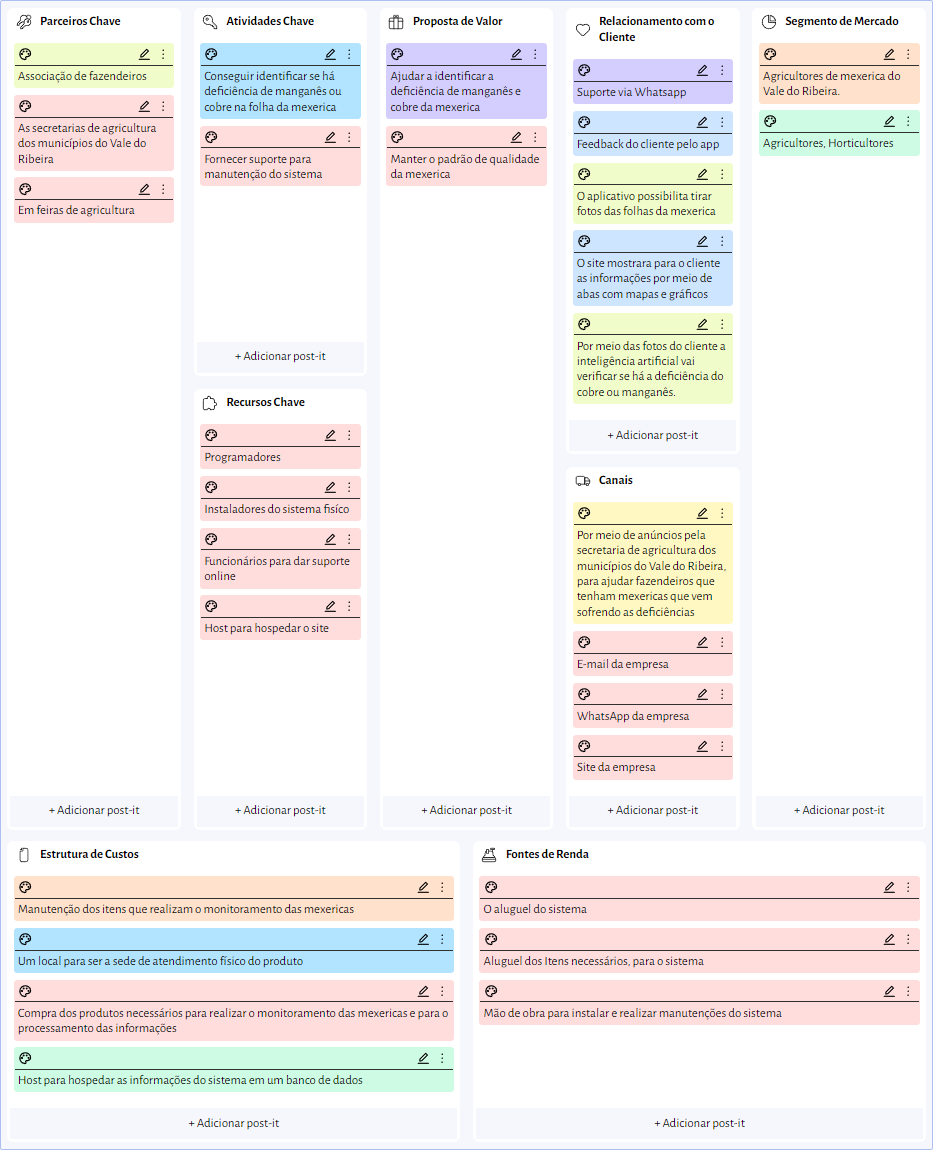
\includegraphics[width=0.8\linewidth]{Illustrations/canvas.png}
    \SourceOrNote{Autoria Própria (2024)}
    \end{figure}
    
\end{Appendix}
    
    
    %% Índice remissivo
\printindex%
    

%%%% Elementos pós-textuais
%%
%% Glossário, apêndices, anexos e índice remissivo (opcionais).

%% Apêndices
\begin{Appendix}

    \section{Modelo de negócios Canvas}%
    \label{sect:apx-a1}
    
    \begin{figure}[H]
    \centering
    \caption{Modelo de negócios Canvas}%
    \label{fig:canvaspi}
    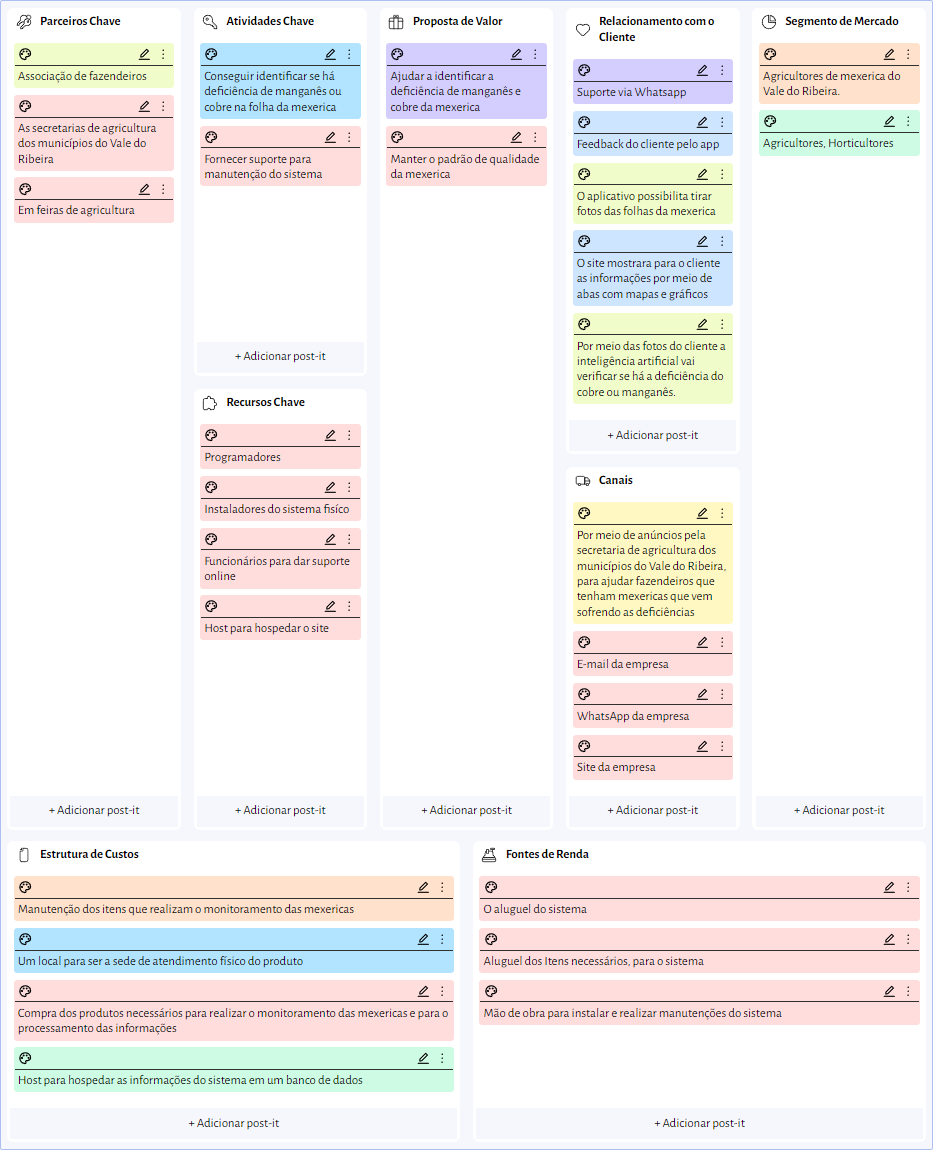
\includegraphics[width=0.8\linewidth]{Illustrations/canvas.png}
    \SourceOrNote{Autoria Própria (2024)}
    \end{figure}
    
\end{Appendix}
    
    
    %% Índice remissivo
\printindex%
    

%% Fim do documento
\end{document}